\chapter{Introduction}

Provenance as a concept has been around for a long time. It originally comes from the Latin word \textit{provenio}, meaning ``to come forth'' and its primary use has been in the field of art and antiques where provenance is used to identify the authenticity and quality of a piece of artwork. For anyone with a background in databases this term may also be familiar as the concept of linking tuples from the output of a query to the reason they exist.

\textit{Digital provenance} is a type of metadata representing the lineage of an object. Naively it can be compared to the information stored in revision history systems like that used in google docs\footnote{Google docs: \url{https://docs.google.com}} or version control
% TODO: git and mercurial links
systems such as git or mercurial\footnote{Git \url{https://git-scm.com/} and mercurial \url{https://www.mercurial-scm.org/}}. These systems are usually limited to storing revisions and authorship. Provenance extends beyond this by making it possible to store and ultimately trace what other entities and activities led to a digital objects current state. By studying the provenance of a file or digital object a user is able to identify what processes, other files and bits of data influenced the file.

Provenance has the potential to be useful in any field where the lineage of an object needs to be stored. One example would be in data warehouse systems where information about data transformations and data origins is stored. Another would be banking or accounting systems where reasearch has been done into preventing provenance forgery through the use of block chains~\cite{Hasan2009}.

The field that is the focus of this paper is that of personal data management, using provenance to  allow users to understand how their data has been used. Often when a user chooses to share their personal data it is aggregated, anonymised or passed through any number of functions. By exploring provenance users have the ability to understand exactly how much and in what state their personal data is used.

An example to illustrate this point. We have a person called Alice. She tracks her steps using a Fit-Bit\footnote{Fitbit is a company that sells wearable devices to track you steps and other fitnes data \url{https://www.fitbit.com/}} and weight using a Withings scale\footnote{Withings sells ditigal scales that can log you weigh information wirelessly and automatically \url{http://www.withings.com/us/en/products/smart-body-analyzer}}. She uses the Fit-Bit dashboard to monitor her progress, it displays a series of summaries related to fitness data as seen in Figure~\ref{fig:fitness-dashboard}. However she wonders how some of this data is calculated, from (B) in Figure~\ref{fig:fitness-dashboard} she had deduced that other people can see her fitness score and she is not comfortable with what information her friends might be able to imply from it (for example, would her friends be able to tell when she has missed her fitness goals?).

\begin{figure}[h]
	\centering
  \begin{subfigure}[t]{0.5\textwidth}
	\label{fig:fitness-dashboard-weight}
    \centering
	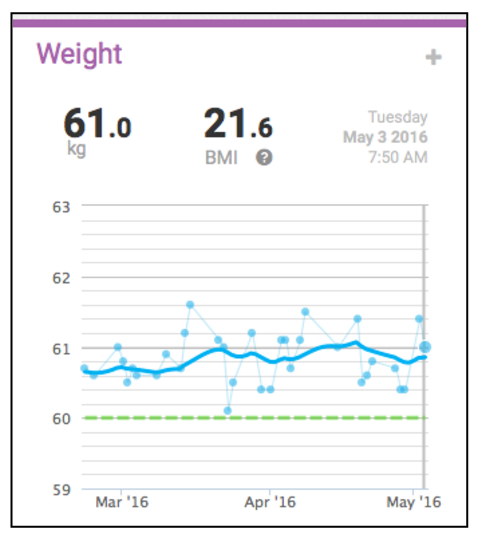
\includegraphics[width=0.8\linewidth]{dashboard1}
    \caption{A summary of Alice's weight data.}
  \end{subfigure}
  \begin{subfigure}[t]{0.4\textwidth}
	\label{fig:fitness-dashboard-score}
    \centering
	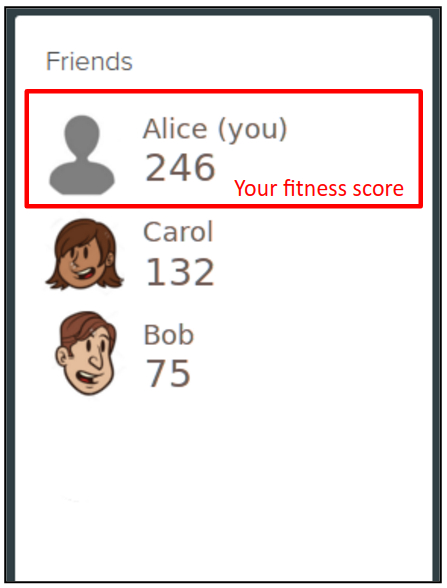
\includegraphics[width=0.8\linewidth]{dashboard2}
    \caption{A display of Alice's current fitness score and the scores of her friends Bob and Carol.}
  \end{subfigure}
  \begin{subfigure}[t]{0.8\textwidth}
	\label{fig:fitness-dashboard-steps}
    \centering
	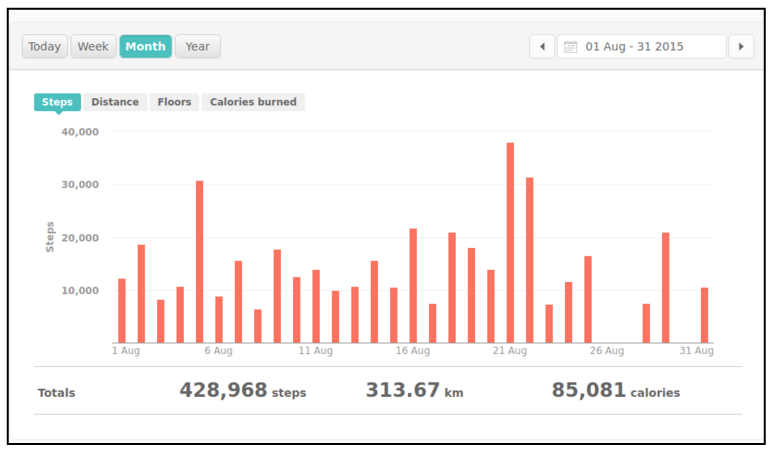
\includegraphics[width=0.8\linewidth]{dashboard3}
    \caption{A summary of Alice's step data.}
  \end{subfigure}

	\caption{Alice's Fitness dashboard shows summaries of information about her. She wonders how some of this information is calculated.}
	\label{fig:fitness-dashboard}
\end{figure}


Luckily Fit-Bit stores the provenance of these summaries, so it is possible to find out what data is used to create each of those in Alice's dashboard. However the provenance is stored in PROVN, a text serialisation that's difficult to read, as seen in Figure~\ref{fig:fitness-score-provn}. Alice, a non technical user, is not surprisingly overwhelmed by this and is no closer to understanding how her fitness score was calculated than before she had access to its provenance.

The industry standard for visualising provenance graphs is through acyclic directed graphs (although some other visualisation techniques have been experimented with~\cite{Borkin2013}). Representing Alice's fitness score provenance this way makes it easier to understand than the raw PROVN file, as seen in dagram (A) of Figure~\ref{fig:fitness-score-dag}. It is now possible to see that across the bottom of the graph is a series of entities attributed to Alice such as \texttt{step\_tracker\_data} and \texttt{step\_goal}. It can also be seen that these entities are somehow used, through a series of activities, as input for her fitness score. However this graph is still too complex for a non technical user and perhaps even a technical user. The next step is to simplify the graph by clustering some of the nodes together to create something like diagran (B) of Figure~\ref{fig:fitness-score-dag}. In this graph I have taken all the nodes related to weight data and step data and created clusters of them both, reducing the graph from having 15 nodes to only five. This makes it much easier to understand and conveys the same core concepts as before except through fewer nodes. We come here to the crux of the problem that my thesis explores: \textit{Provenance graphs are too complex for regular users to understand.}

What we describe in this paper is the design, implementation and evaluation of an interface that enables users to cluster effectively. 
\begin{figure}[b]
	\centering
	\lstinputlisting[style=provn, firstline=3, lastline=10]{misc/fitness-score.provn}
	\caption{A extract of the provenance of Alice's fitness score written in the provn standard. It is quite inweildly to read, even for someone similar with provenance data. View the entire file in~\ref{sec:prov_file_fitness_score}}
	\label{fig:fitness-score-provn}
\end{figure}

\begin{figure}[h]
	\centering
	\begin{subfigure}[t]{\textwidth}
    \centering
	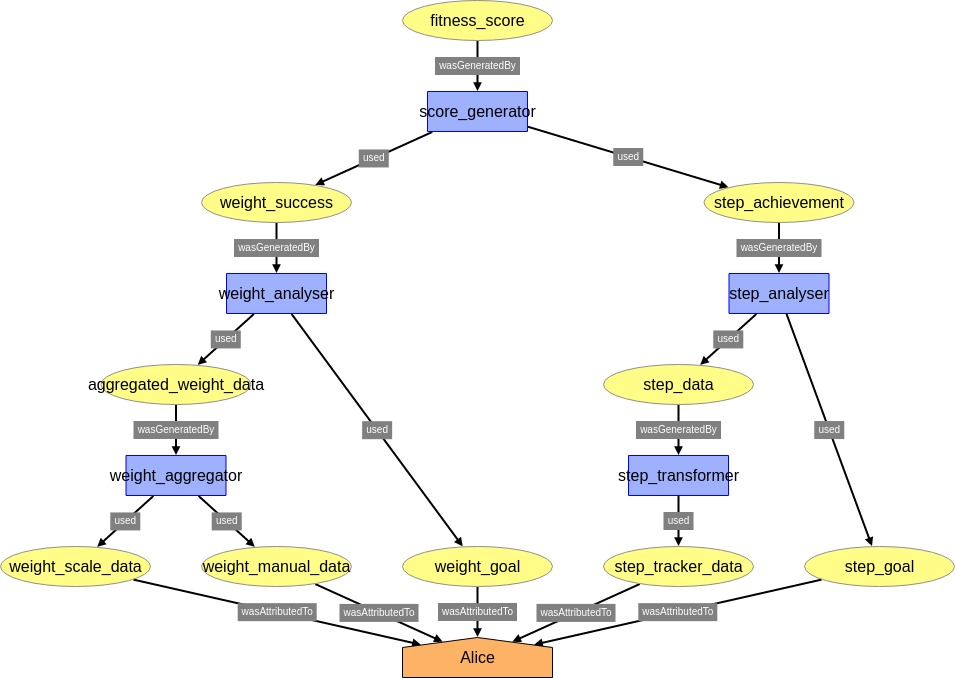
\includegraphics[width=0.8\linewidth]{fitness-score-dag}
    \caption{The provenance of Alice's fitness score represented as an acyclic directed graph.}
  \end{subfigure}
  \begin{subfigure}[t]{\textwidth}
    \centering
	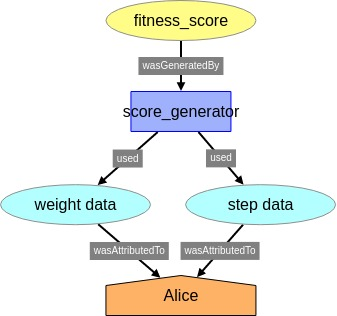
\includegraphics[width=0.4\linewidth]{fitness-score-dag-clustered}
    \caption{The provenance of Alice's fitness score with manually created clusters.}
  \end{subfigure}

	\caption{Two directed acyclic graphs showing the provenance of Alice's fitness score.}
	\label{fig:fitness-score-dag}
\end{figure}

